\documentclass{article}
\usepackage{cmap} % поиск в PDF
\usepackage[T2A]{fontenc} % кодировка
\usepackage[utf8]{inputenc} % кодировка исходного текста
\usepackage[english,russian]{babel} % локализация и переносы
\usepackage[usenames]{color}
\usepackage{colortbl}
\usepackage{url}
\usepackage{amsfonts}
\usepackage{amsmath}
\usepackage{amssymb}
\usepackage{graphicx} %package to manage images
%\graphicspath{ {./images/} }
\usepackage{graphicx}
\usepackage[rightcaption]{sidecap}
\usepackage{wrapfig}
\newcommand{\RNumb}[1]{\uppercase\expandafter{\romannumeral #1\relax}}


\begin{document}

\thispagestyle{empty}

\begin{center}
\ \vspace{-3cm}

{\scshape Московский государственный\\
Ордена Ленина, Ордена Октябрьской Революции,\\
Ордена Красного Трудового Знамени\\
университет имени М.~В.~Ломоносова}\\
Факультет вычислительной математики и кибернетики\\
Кафедра системного анализа

%\vfill
\vspace{1cm}

\includegraphics[width=6, height=6]{mgu}
\vspace{1cm}

{\LARGE Отчёт по практикуму на ЭВМ}

\vspace{1cm}

{\Huge\bfseries <<Реализация преобразования Фурье средствами Matlab>>}
\end{center}

\vspace{1cm}

\begin{flushright}
  \large
  \textit{Студент 315 группы}\\
  А.\,А.~Самойлов

  \vspace{5mm}

  \textit{Руководитель практикума}\\
  к.ф.-м.н., доцент П.\,А.~Точилин
\end{flushright}

\newpage
{\Large\bfseries\section{Постановка задачи}}
Требуется реализовать функцию в~среде Matlab, которая, используя быстрое преобразование Фурье, будет считать аппроксимацию преобразования Фурье
$F(\lambda)$ для~функций:

1) $f_1(t) = \frac{2-t}{1+5t^2}$

2) $f_2(t) = e^{-t^2} \sinh t$

3) $f_3(t) = e^{|t|}\frac{1+2t}{1+t^4}$

4) $f_4(t) = \frac{1-\cos t^2}{t^3}$

\noindent Должна быть реализована возможность выбора шага дискретизации, входного и~выходного окон.
Для первых двух функций требуется посчитать преобразование Фурье в~явном виде и~сравнить графики полученных функций с~графиками их~аппроксимаций.
\vspace{0.5cm}

{\Large\bfseries\section{Теоретические сведения о задаче}}
\noindent$f(t)$ - функция, данная по условию.

\noindent $[a,b]$ - окно функции f(t).

\noindent Оконная функция:
\[
h_{[a,b]}(t) =\begin{cases}
  1, & t \in [a,b] \\
  0, & t \notin [a,b]
\end{cases}
\]
\noident $step$ - шаг дискретизации.
\noident $N$ - число точек множества, на~котором строится функция.
\vspace{0.5cm}

{\Large\bfseries\section{Ход решения}}
\noindent 1) Построим равномерное разбиение отрезка $[a,b]$ по~$N$ точкам

\noindent 2) Пересчитаем шаг дискретизации так, чтобы в~$[a,b]$ входил $N-1$ подотрезок длины 
$\Delta t = \frac{b-a}{N}$, где $N = round(\frac{b-a}{step})$. $\Delta t$ - новый шаг дискретизации.

\noindent 3) Обозначим $\tilde f(t) = f(t)h_{[a,b]}(t)$ и~продолжим ее~по~периоду $b-aч$. Зададим множество, на~котором будет строиться преобразование Фурье:

$\{X_n\} = \{\tilde f(\Delta tn); \ n = \overline{0,N-1}\}$

\noindent 4) Применим к этому множеству БПФ, реализуемое в Matlab функцией fft() и получим множество комплексных отсчетов:

$\{F_n\} = \{\Delta t \cdot \sum\limits_{k=1}^n\tilde f(\Delta tn)e^{-\frac{ikn}{N}};
\ n = \overline{0,N-1}\}$

\noident Частота дискретизации в частотной области преобразования Фурье находится по формуле:

$\Delta f = \frac{2\pi}{b-a}$

\noindent 5) Продлеваем функцию по периоду, разделяем ее вещественную и мнимую части и строим их графики.

\newpage

{\Large\bfseries\section{Аналитическое вычисление преобразования Фурье}}
1) $f(t) = \frac{2-t}{1+5t^2}$
\[
\begin{flushleft}

\noindent F(\lambda) = \int\limits_{-\infty}^{+\infty} \frac{2-t}{1+5t^2}e^{-i\lambda t}\,dt = 
\int\limits_{-\infty}^{+\infty} \frac{2-t}{(1+i\sqrt{5}t)(1-i\sqrt{5}t)}e^{-i\lambda t}\,dt

\end{flushleft}
\]
$t_1 = -\frac{1}{i\sqrt{5}}, t_2 = \frac{1}{i\sqrt{5}}$ - полюса \RNumb{1} порядка.

\noindentБудем искать значение интеграла через вычеты.
\vspace{-0.7cm}
\[
\begin{flushleft}
res\limits_{t = t1} =  \lim\limits_{t \to t1}(t+\frac{1}{i\sqrt{5}})
\frac{2-t}{(1+i\sqrt{5}t)(1-i\sqrt{5}t)}e^{-i\lambda t} = 
\lim\limits_{t \to t1}\frac{2-t}{i\sqrt{5}(1-i\sqrt{5}t)}e^{-i\lambda t} = \frac{2+\frac{1}{i\sqrt{5}}}{i2\sqrt{5}}e^{\frac{\lambda}{\sqrt{5}}}
\end{flushleft}
\]
\vspace{-1.8cm}
\[
\begin{flushleft}
res\limits_{t = t2} =  \lim\limits_{t \to t1}(t-\frac{1}{i\sqrt{5}})
\frac{2-t}{(1+i\sqrt{5}t)(1-i\sqrt{5}t)}e^{-i\lambda t} = 
\lim\limits_{t \to t2}\frac{t-2}{i\sqrt{5}(1+i\sqrt{5}t)}e^{-i\lambda t} = \frac{\frac{1}{i\sqrt{5}}-2}{i2\sqrt{5}}e^{\frac{-\lambda}{\sqrt{5}}}
\end{flushleft}
\]
\vspace{-1.6cm}
\[
\begin{flushleft}
F(\lambda) = 2\pi i\begin{cases}
  res\limits_{t = t1}, & \lambda < 0 \\
  res\limits_{t = t2}, & \lambda > 0
\end{cases}
= \begin{cases}
  \frac{\pi e^{-\frac{\lambda}{\sqrt{5}}}}{\sqrt{5}}(\frac{1}{i\sqrt{5}}-2), & \lambda < 0 \\
  \frac{\pi e^{\frac{\lambda}{\sqrt{5}}}}{\sqrt{5}}(\frac{1}{i\sqrt{5}}+2), & \lambda > 0
\end{cases}
= \begin{cases}
  \frac{\pi e^{-\frac{\lambda}{\sqrt{5}}}}{5\sqrt{5}}(10+i\sqrt{5}), & \lambda < 0 \\
  \frac{\pi e^{\frac{\lambda}{\sqrt{5}}}}{5\sqrt{5}}(10-i\sqrt{5}), & \lambda > 0
\end{cases}
\end{flushleft}
\]
2) $f(t) = e^{-t^2} \sinh t $
\[
\begin{flushleft}

\noindent F(\lambda) = \int\limits_{-\infty}^{+\infty} e^{-t^2}(\frac{e^t-e^{-t}}{2})e^{-i\lambda t}\,dt =
\frac{1}{2}\int\limits_{-\infty}^{+\infty}e^{-t^2+t}e^{-i\lambdat}\,dt-
\frac{1}{2}\int\limits_{-\infty}^{+\infty}e^{-t^2-t}e^{-i\lambda t}\,dt = \\
=\lbrace u = t - \frac{1}{2};\ v = t+\frac{1}{2}\rbrace = 
\frac{e^{\frac{1}{4}}}{2}\int\limits_{-\infty}^{+\infty}e^{-u^2}e^{-i\lambda (u+\frac{1}{2}})\,du - \frac{e^{\frac{1}{4}}}{2}\int\limits_{-\infty}^{+\infty}e^{-v^2}e^{-i\lambda (v-\frac{1}{2}})\,dv = \\
=\(\frac{e^{\frac{1}{4}-\frac{i\lambda}{2}}}{2}\)\int\limits_{-\infty}^{+\infty}e^{-u^2}e^{-i\lambda u}\,du -
\frac{e^{\frac{1}{4}+\frac{i\lambda}{2}}}{2}\int\limits_{-\infty}^{+\infty}e^{-v^2}e^{-i\lambda v}\,dv = \\
=\lbrace g(t) = e^{-t^2} => G(\lambda) = \frac{1}{\sqrt{2}}e^{\frac{-\lambda^2}{4}}\rbrace = 
\frac{\sqrt{\pi}}{2}(e^{-\frac{\lambda^2}{4}}e^{\frac{1}{4}}(e^{-\frac{i\lambda}{2}}-e^{\frac{i\lambda}{2}}))
= \\ = \sqrt{\pi}e^{\frac{1}{4}+\frac{\lambda^2}{4}}(\cos(-\frac{\lambda}{2})+i\sin(-\frac{\lambda}{2})-
\cos(\frac{\lambda}{2})-i\sin(\frac{\lambda}{2})) =
-i\sqrt{\pi}e^{\frac{1}{4}+\frac{\lambda^2}{4}}\sin\frac{\lambda}{2}
\end{flushleft}
\]

\newpage

{\Large\bfseries\section{Построение Фурье-образов}}
{\large\subsection{$f_1(t) = \frac{2-t}{1+5t^2}$}}
\begin{center}
  $\Delta t = 0.4,\ a = -10,\ b = 10$
  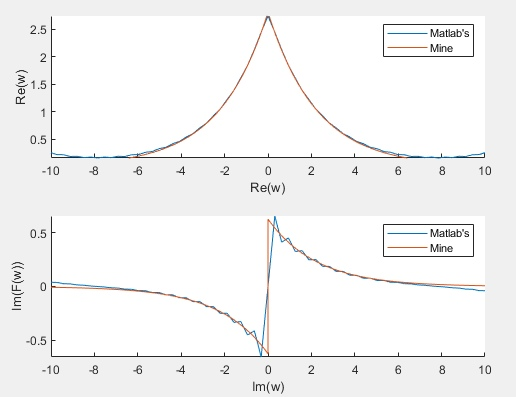
\includegraphics[width = 10cm, height 10cm]{f1_1.jpg}
  \vspace{1cm}
  
  $\Delta t = 0.001,\ a = -100,\ b = 100$
  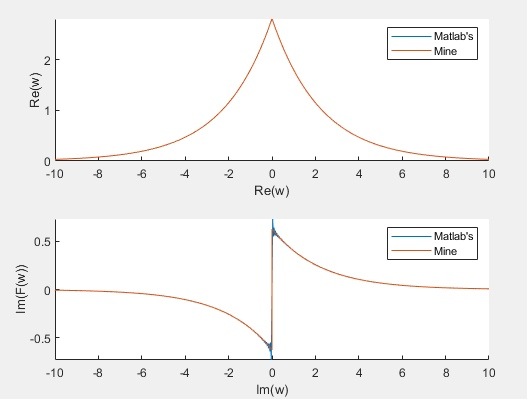
\includegraphics[width = 10cm, height 10cm]{f1_2.jpg}
\end{center}

\newpage

{\large\subsection{$f_2(t) = e^{-t^2} \sinh t$}}
\begin{center}
  $\Delta t = 0.4,\ a = -6,\ b = 6$
  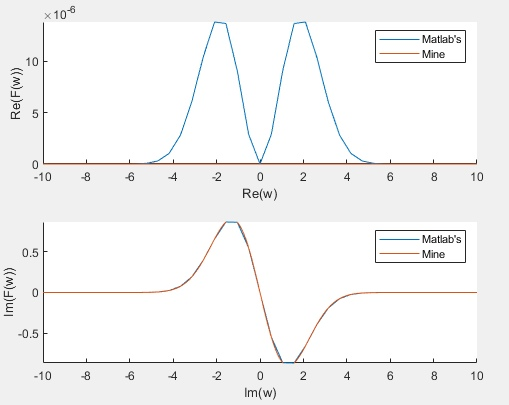
\includegraphics[width = 10cm, height 10cm]{f2_1.jpg}
  \vspace{1cm}
  
  $\Delta t = 0.001,\ a = -100,\ b = 100$
  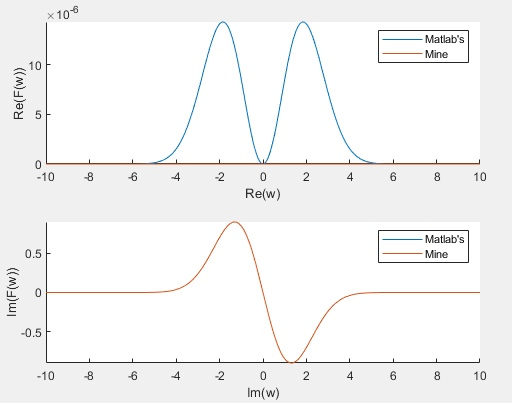
\includegraphics[width = 10cm, height 10cm]{f2_2.jpg}
\end{center}

\newpage

{\large\subsection{$f_3(t) = e^{|t|}\frac{1+2t}{1+t^4}$}}
\begin{center}
  $\Delta t = 0.4,\ a = -4,\ b = 4$
  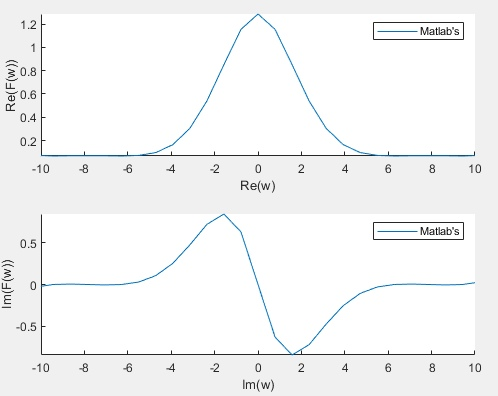
\includegraphics[width = 10cm, height 10cm]{f3_1.jpg}
  \vspace{1cm}
  
  $\Delta t = 0.001,\ a = -100,\ b = 100$
  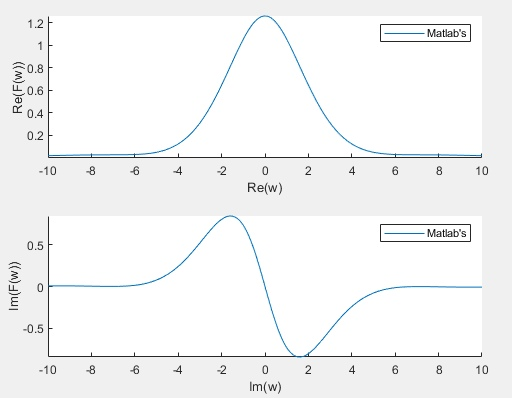
\includegraphics[width = 10cm, height 10cm]{f3_2.jpg}
\end{center}

\newpage

{\large\subsection{$f_4(t) = \frac{1-\cos t^2}{t^3}$}}
\begin{center}
  $\Delta t = 0.1,\ a = -10,\ b = 10$
  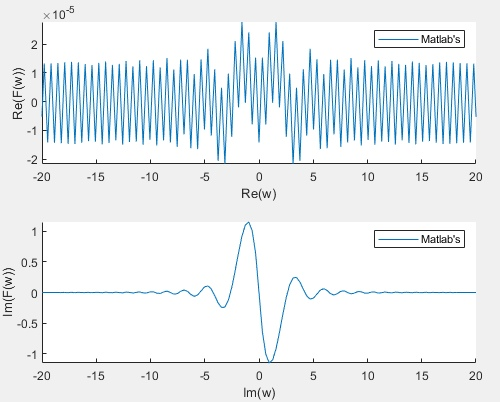
\includegraphics[width = 10cm, height 10cm]{f4_1.jpg}
  \vspace{1cm}
  
  $\Delta t = 0.001,\ a = -100,\ b = 100$
  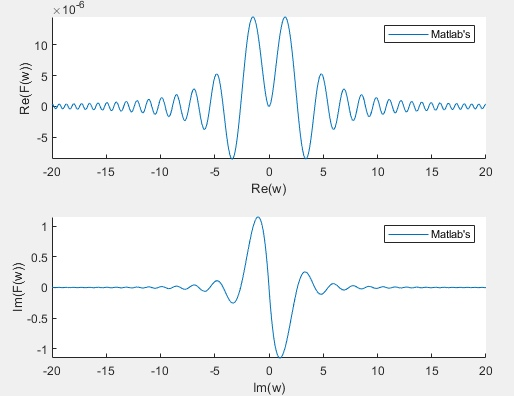
\includegraphics[width = 10cm, height 10cm]{f4_2.jpg}
\end{center}

\newpage

  
{\Large\bfseries\section{Эффект наложения спектра и его \\ устранение}}
\noindent Для иллюстрации данного эффекта выберем 1 функцию, и~сравним кривую аналитичкского решения(синяя) с двумя кривыми аппроксимаций(красные).

{\large\subsection{Сильное наложение, вызвоное большим шагом дискретизации:}}
\begin{center}
  $\Delta t = 0.5,\ a = -10,\ b = 10$
  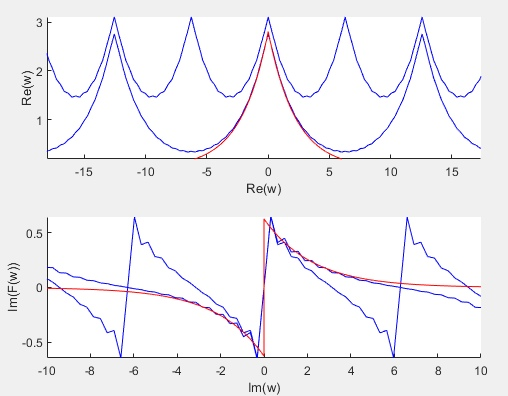
\includegraphics[width = 12cm, height 12cm]{spectre2_1.jpg}
\end{center}

{\large\subsection{Улучшение ситуации при уменьшении шага дискретизации:}}
\begin{center}
  $\Delta t = 0.2,\ a = -10,\ b = 10$
  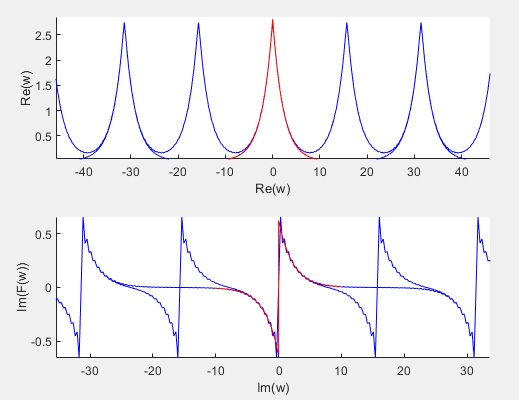
\includegraphics[width = 12cm, height 12cm]{spectre2_2.jpg}
\end{center}

{\large\subsection{Исчезновение эффекта наложения при последующем уменьшении шага дискретизации:}}
\begin{center}
  $\Delta t = 0.01,\ a = -10,\ b = 10$
  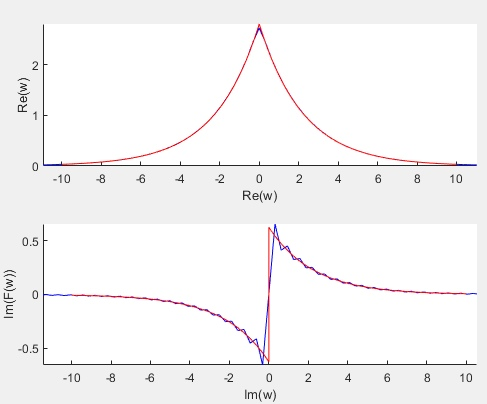
\includegraphics[width = 12cm, height 12cm]{spectre2_3.jpg}
\end{center}

\newpage

{\Large\bfseries\section{Рябь и ее~минимизация:}}
\noindent Для иллюстрации ряби выберем график первой функции, так~как~у~нее есть рябь в окрестности нуля в силу наличия в нуле разрыва \RNumb2 рода.

{\large\subsection{Сильная рябь при малом окне функции:}}
\begin{center}
  $\Delta t = 0.01,\ a = -10,\ b = 10$
  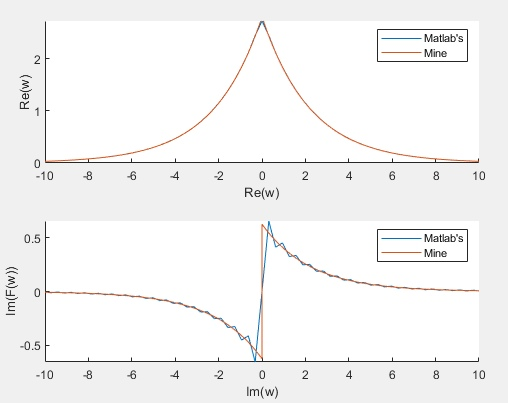
\includegraphics[width = 12cm, height 12cm]{dribble_1.jpg}
\end{center}

{\large\subsection{Уменьшение ряби при увеличении окна функции:}}
\begin{center}
  $\Delta t = 0.01,\ a = -30,\ b = 30$
  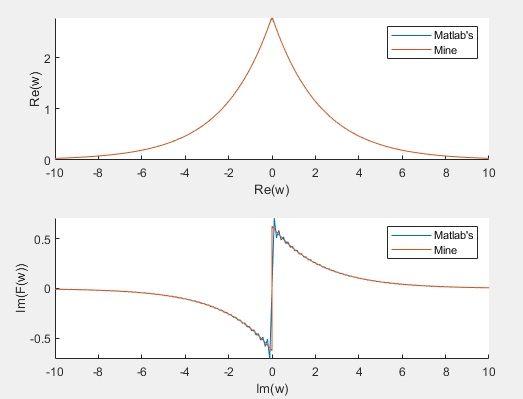
\includegraphics[width = 12cm, height 12cm]{dribble_2.jpg}
\end{center}

{\large\subsection{Последующее уменьшение ряби при дальнейшем увеличении окна функции:}}
\begin{center}
  $\Delta t = 0.01,\ a = -1000,\ b = 1000$
  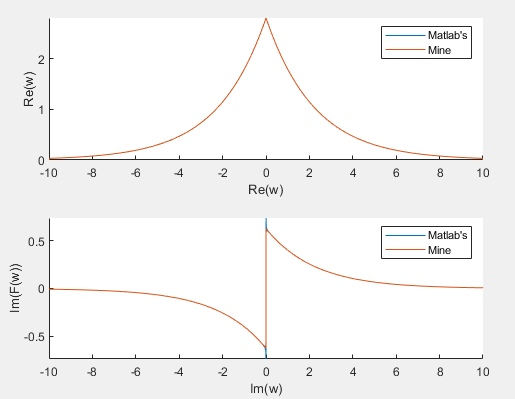
\includegraphics[width = 12cm, height 12cm]{dribble_3.jpg}
\end{center}
\noindent К сожалению, в точках разрыва \RNumb2 рода полностью устранить рябь не получается, но можно свести ее визуальное присутствие к $\varepsilon$-окресности точки разрыва для любого $\varepsilon > 0$ путем увеличения окна функции.

\end{document}